\documentclass[paper=a4, fontsize=12pt]{scrartcl}

\usepackage[T1]{fontenc}
\usepackage[english]{babel}
\usepackage{amsmath,amsfonts,amsthm}
\usepackage{fancyhdr}
\pagestyle{fancyplain}
\fancyhead{}
\fancyfoot[L]{}
\fancyfoot[C]{}
\fancyfoot[R]{\thepage}
\renewcommand{\headrulewidth}{0pt}
\renewcommand{\footrulewidth}{0pt}
\setlength{\headheight}{13.6pt}
\usepackage[margin=1in]{geometry}
\usepackage{graphicx}
\graphicspath{ {images/} }

%\setlength\parindent{0pt}

\newcommand{\horrule}[1]{\rule{\linewidth}{#1}}

\title{
\normalfont \normalsize
\textsc{PV204} \\ [25pt]
\horrule{0.5pt} \\[0.4cm]
\huge Project 2: Review  \\
\horrule{2pt} \\[0.5cm]
}

\author{Roman Kollar, Rajesh Kumar Pal,\\Himanshu Kumar Haran, Ameet Kumar Haware}
\date{\normalsize\today}
\begin{document}
\maketitle

\section{Introduction}
\subsection{Secure channel}
The design document states that there will be a secure channel between the card and the application using encryption, session keys and HMAC.
However, there is no code that implements any of those
For example, the PIN in the verification process is sent in plain and could be intercepted.

The secret data stored on the card are sent encrypted but with a static (hardcoded) key and IV which adds no security.
Even if every client had its own application with randomly generated key, storing the key this way makes the application completely unsecure.

The application does not authenticate the applet in any way and the card could be replaced by a malicious one.
And since the applet uses same AID as the SimpleAppet from class, even the SimpleApplet loaded on the card works for generating passwords.

The security improvement of using this implementation is therefore questionable.
% TODO: but it IS using random number generator of the javacard

\subsection{Slots}
The authenticated state was supposed to be tied to an unique string indentifier of the data stored on the card.
However, this is not true.
The entire applet is either authenticated or not.
Access to "slots" is implemented using the \verb@P1@ parameter in the APDU.
There is no authorization when getting data from the card.
An attacker can access all the data (which is encrypted with the same key) just by changing the \verb@P1@ parameter.

Also note that changing the pin changes the global pin, not a pin tied to any identifier.

\section{JPass}
PC-App sends encrypted password to Javacard. %%% Roman: please write more about this or I will have to rewrite it
%The encryption is done by some default key in the pc-app ( yet to be find out ) %%% Roman: this is already explained in the Secure channel part

\subsection{Compilation}
Without any changes, compilation does not work with any of the two suggested tools.
\verb@Maven@ works after adding dependency for \verb@jcardsim@.

\subsection{Testing}
The modified application works.
However, only generating passwords works using a smart card.
Trying to save or load data ends with an error:

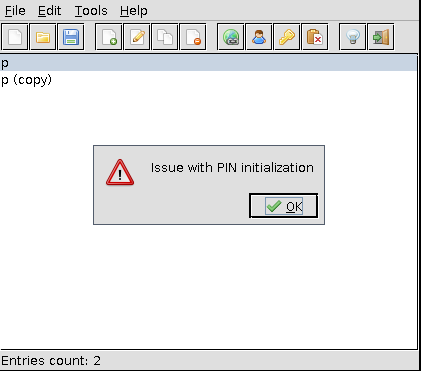
\includegraphics[scale=0.5]{jpass_error}

\subsubsection{Static analysis}
% TODO


\section{JPass Applet}
JavaCard stores the password and other metadata.
%There is no secure channel (This point was told by them in their ppt). %%% Roman: this is also already explained in the secure channel part, please read that first...also, what ppt? there is only a pdf in the zip file and says there IS a secure channel

\section{Conclusion}

\end{document}
